
\documentclass[12pt]{report}

%  PACKAGES ==========================================================
\usepackage{amsmath,amsthm,amsfonts,amssymb,amscd,mathrsfs,mathtools}  % Math packages
\usepackage{natbib}         % for references
\usepackage{multirow}       % for equaitons
\usepackage{wrapfig}        % to wrap figure with text
\usepackage{graphicx}       % allows adding graphics to the text
\usepackage{verbatim}       % Allows quoting source with commands.
\usepackage{makeidx}        % Package to make an index.
%\usepackage{psfig}          % Allows inclusion of eps files.
%\usepackage{epsfig}         % Allows inclusion of eps files.
%\usepackage{epstopdf}       % allows .eps figures in the text
%\usepackage{pdftex}        % allows .eps figures in the text
%\usepackage{pdflatex}      % allows .eps figures in the text

\usepackage{url}            % Allows good typesetting of web URLs.
\usepackage{subfigure}      % to have multi figures in the same figure
\usepackage{comment}        % allow commnets in the file
%\usepackage[linesnumbered,lined,boxed,commentsnumbered]{algorithm2e} % To include algorithm - this one is more professional, but we cannot break the algorithm in pages
\usepackage{float}
%\usepackage{algorithm}      % To include algorithm
%\usepackage{algpseudocode}  % for algorithms
\usepackage[bookmarks]{hyperref}  % to add bookmarks to all references
\usepackage{ragged2e}       % Text justifying
\usepackage{color}
\usepackage{ctable}
%\usepackage{pmat}
%\usepackage{ulem}
%\usepackage[retainorgcmds]{IEEEtrantools}
%\usepackage[dvips]{geometry}
%\usepackage{lscape}
%\setcounter{MaxMatrixCols}{40}

%\usepackage[framed,numbered,autolinebreaks,useliterate]{mcode} % Add a Matlab code
%\usepackage{eucal} 		    % Euler fonts
%\usepackage{setspace}
%\usepackage{algorithm,algorithmicx,algpseudocode}   % algorithms
%\usepackage{draftcopy}		% Uncomment this line to have the
                          %   word, "DRAFT," as a background
                          %   "watermark" on all of the pages of
                          %   of your draft versions. When ready
                          %   to generate your final copy, re-comment
                          %   it out with a percent sign to remove
                          %   the word draft before you re-run
                          %   Makediss for the last time.

% Extra stuff =======================================================
%\allowdisplaybreaks  % to break long equations into two pages


% = Constants ========================================================
\renewcommand\textfraction{.1}
\setcounter{totalnumber}{5}
\renewcommand{\floatpagefraction}{.8}

%\setlength{\bibsep}{0pt plus 0.3ex}    % This line reduces the spacing between the references  - Remove in the final version

% = Figure spacing ==================================================
\renewcommand{\subfigbottomskip}{-2pt}
\renewcommand{\subfigcapskip}{-2pt}
\renewcommand{\subfigcapmargin}{0pt}

%\setlength{\belowcaptionskip}{-10pt}

\setlength{\textfloatsep}{14pt plus 1.0pt minus 2.0pt}
\setlength{\intextsep}{14pt plus 1.0pt minus 2.0pt}
\setlength{\floatsep}{14pt plus 1.0pt minus 2.0pt}


% General information ===============================================
\author{Babak Poursartip}
%\address{babakp@utexas.edu}

\title{My ML studies}

\makeatletter		% Starts section where @ is considered a letter
          			% and thus may be used in commands.
\def\square{\RIfM@\bgroup\else$\bgroup\aftergroup$\fi
  \vcenter{\hrule\hbox{\vrule\@height.6em\kern.6em\vrule}%
                                              \hrule}\egroup}
\makeatother		% Ends sections where @ is considered a letter.
			          % Now @ cannot be used in commands.

%\makeindex      % Make the index


% Beginning =========================================================
\begin{document}

\justifying


%\titlepage    % Produces the title page.
\maketitle



% Tables ============================================================
\pdfbookmark{\contentsname}{toc}  % To bookmark the table of contents
\tableofcontents                  % Table of Contents will be automatically
%\listoftables                     % List of Tables and List of Figures will be placed
%\listoffigures                    % here, if applicable.
%\listofalgorithms                 % List of algorithms
%\addcontentsline{toc}{chapter}{List of Algorithms}  % This command includes the list of algorithms in the table of content

% Chapters =====================================================================
%===============================================================================
%===============================================================================
%===============================================================================
%\include{chapter1_Introduction}
\chapter[Introduction]{Introduction to ML}
\label{ch:ML}
\noindent

\section{General}

\begin{itemize}
	\item Supervised learning (SL): functional approximation from labeled data.
	\item Unsupervised learning (UL): functional description. Learning from unlabeled data.
	\item Reinforcement learning (RL): Learning from delayed reward.
\end{itemize}






%===============================================================================
%===============================================================================
%===============================================================================
\chapter[Supervised learning]{Supervised learning (SL)}
\label{ch:sl}
There are two types of supervised learning:

\begin{itemize}
\item classification: taking some inputs and mapping it to some discrete labels. (true of false; male or female; SUV or sedan or truck; class1, class2, class3.)
\item regression: returns continuous valued function. Mapping from input to some \textbf{real number}. Something like age is more like discrete number, so, it is also classification.
\end{itemize}

\section{Terms}
\begin{itemize}
\item Instances: Inputs, such as pictures, pixels, etc.
\item Concept: A set of \textit{functions} that maps inputs to outputs.
\item Target concept: The actual function that can map inputs to outputs. This is the actual answer.
\item Hypothesis class: Set of all the functions that we are going to think about.
\item Sample (Training set): A set of instances with correct labels.
\item Candidate: The best approximation of the target concept.
\item Testing set: A set of instances with correct labels that was not visible to the learning algorithm during the training phase. It’s used to determine the algorithm performance on novel data. we can argue that we learned something by memorization, but indeed, we just memorized the concepts. What we want is generalization.
\end{itemize}


\section{SL: Decision tree}

\subsection{Introduction}

Decision tree is a classification learning in the form of a sequence of decisions based on the attributes/features/questions (which forms the nodes) applied to every instance to assign it to a specific class. Answers to the questions would be the edges of the trees.
For example, deciding to eat at a restaurant or not, or classification of vehicles into sedans, SUVs, trucks, etc.

\subsection{Representation of the decision tree:}

A decision tree is a structure of nodes, edges and leaves that can be used to \textit{represent} the data. We always start at the root of the tree, otherwise we don't look at any other attribute in the tree.
\begin{itemize}
\item Nodes represent attributes where you ask a question about it. (vehicle length, vehicle height, number of doors, etc.).
\item Edges represent values/answers, a specific value for each attribute/question.
\item Leaves represent the output (or final answer). For example, vehicle’s type.
\end{itemize}

\subsection{Algorithm to build a decision tree}
Algorithm means how to create the decision tree. A decision tree \textit{algorithm} is a sequence of steps that will lead you to the desired output. To form a decision tree, we need to come up with the attributes that can split the space, roughly in half.
\begin{itemize}
\item Pick the best attribute (the one that can split the data roughly in half). If this attribute added no valuable information (not a good split), it might cause overfitting.
\item Ask a question about this attribute.
\item Follow the correct answer path.
\item Loop back to (1) till you narrow down the possibilities to one answer (the output).
\end{itemize}
Note that the usefulness of a question depends upon the answers we got to previous questions.

Purity: means all the samples are of the same kind. This is the ideal case for the leaf nodes. We have impurity if it is still a mix of various categories.

\subsection{Expressiveness}

\begin{itemize}
	\item Decision trees can basically express any function using the input attributes.
	\item For Boolean functions (AND, OR, XOR, etc.), the truth table row will be translated into a path to a leaf.
	\item How many decision trees we can generate for a specific function/problem? For n boolean attributes with boolean output, the decision tree hypothesis space is very huge $(2^{(2^{n})})$. (Babak note:  this number of decision tree is not really distinct, see my notebook).
	This is why we need to design algorithms to efficiently search the hypothesis space for the best decision tree.
\end{itemize}

Decision trees with AND and OR are linear (they need linear number of nodes-ANY type problems). But XOR is a hard problem (requires $2^n$ nodes-PARITY type of problems).

\subsection{ID3 algorithm to create a decision tree}
We need to find the best attributes for each node, to narrow down the space with each question.
ID3 (Inducing Decision Tree (3)) builds decision trees using a top-down, greedy approach. The greedy part of the approach comes from the fact that it will decide which attribute should be at the root of the tree by looking just one move ahead. It compares all available attributes to find which one classifies the data the best, but it doesn't look ahead (or behind) at other attributes to see which combinations of them classify the data the best. ID3 algorithm returns an optimal decision tree, but as the size of the training data and the number of attributes increase, it becomes more likely that running ID3 on it will return a suboptimal decision tree.

\hfill \break
\textbf{To train a decision tree, answer these questions:}
\begin{itemize}
	\item How to find the best attribute/feature for the decision tree at each level?
	\item When do you stop splitting?
\end{itemize}

\hfill \break
\textbf{Pseudo code:}
\begin{enumerate}
\item Pick the best attribute A (the definitions of best attribute comes later). To select this attribute, a statistical test is used to determine for each attribute how well it alone classifies the training examples.
\item Split the data into subsets that correspond to the possible values of the best attribute.
\item Assign A as a decision attribute for a node.
\item For each value of A, create a descendant node.
\item Sort training examples to leaves.
\item Stopping criteria (see down there): f examples perfectly classified (means all data point are of the same class) or there is no more attributes --	Stop splitting -- else --Iterate over leaves
\end{enumerate}

\hfill \break
\textbf{How to find the best attribute/feature for the decision tree at each level:} \\
There are a couple of options. The most common method is called information gain: a measure that expresses how well an attribute splits the data into groups based on classification (maximize purity or minimize impurity). For example, an attribution returns \textit{low information gain}, if it divides samples to two classes with an even yes and no, but the information gain is high, if each class has more of yeses or nos.

It quantifies the reduction in randomness (Entropy) over the labels we have with a set of data, based upon knowing the value of a particular attribute. A mathematical way to measure the gain, is entropy. It measures the homogeneity of a data set S's  classifications. \textcolor{red}{\textit{Entropy ranges from 0, which means that all of the classifications in the data set are the same (either yes or no), to $log_{2}$ of the number of different classifications, which means that the classifications are equally distributed within the data set.}} For a binary classification the entropy is only $log_{2} 1 = 1$ (if yes and no samples are equally divided). entropy is calculated as follows:

\begin{equation}
Entropy(S) = \sum_{i=1}^{c} -p_{i} \; log_{2} (p_{i})
\end{equation}
where:
\begin{itemize}
\item $c$ corresponds to the number of different classifications (either for the attribute or the final output)
\item $p_{i}$ corresponds to the proportion of the data with the classification i
\end{itemize}

Here is the plot of entropy for a binary classifier, as the proportional of yes and no samples change:


\begin{figure}[H]
	\centering
	\caption{Entropy}
	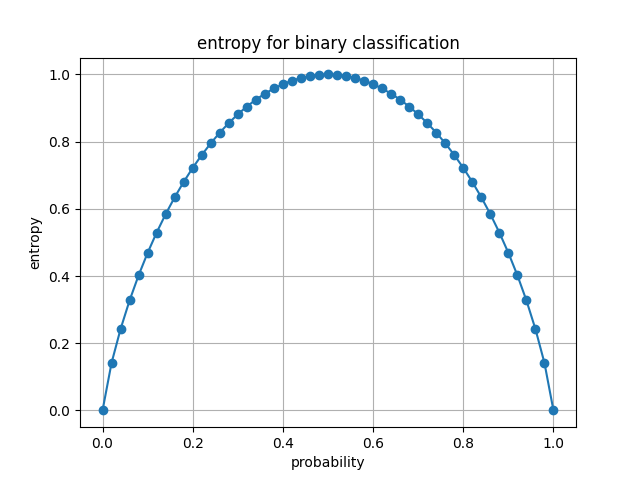
\includegraphics[scale=0.5]{entroy.png}
	%{\footnotesize\textbf{Notes:} XXX.} % changed <<<<<<<<<<
	%#\label{XXX}
\end{figure}




Information gain measures the reduction in entropy that results from partitioning the data on an attribute A, which is another way of saying that it represents how effective an attribute is at classifying the data. Given a set of training data S and an attribute A, the formula for information gain is:

\begin{equation}
	Gain(S,A)  = Entropy(S) - \sum_v  \frac{|S_v|}{|S|} \; Entropy(S_v)
\end{equation}


where $v$ is all the possible values of attribute the attribute (for example, sunny, cloudy, rainy), and $S_v$ is the total number of samples corresponding to this value of attribute (for example sunny).

For \textit{if I play tennis game} (yes and no is the final output) with attributes weather (sunny, cloudy, rainy), temperature (hot, cold, mild), humidity (normal, high),  first, we calculate the entropy of the entire set (Entropy(S)) (wrt the the final output classification, yes and no). For each attribute, we calculate the the entropy corresponding to each value of entropy, then we calculate the final entropy.


We want to maximize information gain, so we want the entropies of the partitioned data to be as low as possible, which explains why attributes that exhibit high information gain split training data into relatively heterogeneous groups.

As the size of the training data and the number of attributes increase, it becomes likelier that running ID3 on it will return a sub-optimal decision tree.


The other option we can use instead of Entropy is the \textbf{Gini function.}

\hfill \break
\textbf{When do you stop splitting?}
\begin{itemize}
	\item when a node is 100\% pure
	\item when splitting a node will result in the tree exceeding a maximum depth (to avoid over-fitting)
	\item when improvement in purity score (information gain) are below a threshold
	\item when the number of examples in a node is below a threshold
\end{itemize}

\subsection{Inductive bias}
Two types of bias for classifiers:
\begin{itemize}
	\item Restriction Bias: Describes the hypothesis set space (H) that we will consider for learning the tree.
	Complete hypothesis space (low Restriction Bias). Instead of looking at infinitely many functions, we only consider those that can be represented by the decision tree.
	\item Preference Bias: Describes the subset of hypothesis n ($n \in H $), from the hypothesis set space H, that we prefer.
\end{itemize}

Inductive bias of ID3 algorithm:
\begin{itemize}
\item it prefers the decision tree with good splits at top (even if a bad split generates the same outcome). This is because ID3 is greedy using info gain.
\item it prefers correct outcome over incorrect because ID3 repeats until the labels are correctly classified.
\item it prefers shorter trees (comes from the fact that we use good splits from the top).
\end{itemize}

\subsection{Extending ID3 algorithm-other consideration}
\textbf{For continuous values attributes/features}, we can classify the attributes based on thresholds (that exists in the data set). Without threshhold, the continuous data attribute provides the most information gain, while giving a decision tree that is not generalize well. To find the threshold, we can plot the values and decide based on a threshold the returns the best outcome, by calculating the information gain values for each threshold. One way to select the threshold is to take all the values that are mid points between the sorted list of training. For example, for 10 training samples, we need to test the info gain for 9 values, for this specific feature. We can even have multiple threshold for one feature (by creating multiple features).

\textbf{Does it make sense to repeat an attribute along a path in a decision tree?} No, it does not make sense for discrete values, but for continuous values, it makes sense, because indeed we are asking a different question (for a different range).

\textbf{If the data for some attributes is missing,} we can choose the most popular data for the missing item. Two options here: does not take the classification into account, or choose the most popular value for the same classification.
Another method to deal with the missing data, is assigning the probability of each value of the attribute to the missing entries.

\textbf{Over-fitting + When do we stop?} When everything classified correctly or if there is no more attribute. What if we have noise in data (different answer for the same instance)? Causes an infinite loop. What would be the stopping criterion, then? We want generalization, and we should avoid \textbf{over-fitting}. If the tree is too big/complicated, there is a chance that it overfits. There are two popular approaches to avoid over-fitting in decision trees: stop growing the tree before it becomes too large or prune the tree after it becomes too large. Typically, a limit to a decision tree’s growth will be specified in terms of the maximum number of layers, or depth, it’s allowed to have.

One option to avoid over-fitting, is that we can grow the trees, and use cross-validation to prevent over-fitting. The data available to train the decision tree will be split into a training set and validation/test set and we keep growing the tree with various maximum depths will be created based on the training set and then test it against the test set. The best will be selected (when the error grows, we stop growing the tree).

Pruning the tree, on the other hand, involves testing the original tree against pruned versions of it. Leaf nodes are taken away from the tree as long as the pruned tree performs better against test data than the larger tree.


\textbf{One-hot encoding:} If there are multiple categories for a feature, we can use one-hot encoding to convert each category to a binary feature. Thus, jf a feature can take k values, one-hot encoding creates k binary features. There are libraries in the sklearn library for this task. See the details in the \ref{sec:one-hot}.

\textbf{Regression:} how to adapt decision trees for regression type of problems (continuous outputs)? Decision trees as we’ve defined them here don’t transfer directly to regression problems. We no longer have a useful notion of information gain, so our approach at attribute sorting falls through. Instead, we can rely on purely statistical methods (like variance and correlation) to determine how important an attribute is. For leaves, too, we can do averages, local linear fit, or a host of other approaches that mathematically generalize with no regard for the meaning of the data.

\subsection{Regression with Decision tree}

We can use decision trees for classification (DecisionTreeClassifier) or for regression (DecisionTreeRegressor). Training a regressor is not any different from the classifier, but for the leaf node, we use the average of the continuous values of all the samples in that node.

The major difference here is that how you choose to split the data at the node. Instead of maximizing the entropy, we try to minimize the variance of the values for the continuous feature. Thus, we calculate the variance for the values at each leaf separated by the feature, then we use a weighted method to combine it.

\begin{multline}
	\text{minimize the variance (means choose the feature with largest value)} = \\
	\text{variance of all samples at the root} - \\
	\big[ \\
	\frac{\text{num of samples in the left leaf}}{ \text{num of total samples }} \times \text{variance of left leaf} +\\
	\frac{\text{num of samples in the right leaf}}{ \text{num of total samples }} \times \text{variance of right leaf}\\
	\big]
\end{multline}



For example, if a feature divides 10 samples into two leaf nodes with 4 and 6 samples in each leaf node, then, the weighted average of variance is $\frac{4}{10} \times \text{variance of left leaf} + \frac{6}{10} \times \text{variance of right leaf} $.

\subsection{Changing the information gain formula is another option}
The information gain formula used by the ID3 algorithm treats all of the variables the same, regardless of their distribution and their importance. This is a problem when it comes to continuous variables or discrete variables with many possible values because training examples may be few and far between for each possible value, which leads to low entropy and high information gain by virtue of splitting the data into small subsets, but results in a decision tree that might not generalize well.

One successful approach to deal with this is using a formula called GainRatio in the place of information gain. GainRatio tries to correct for information gain’s natural bias toward attributes with many possible values by adding a denominator to information gain called SplitInformation. SplitInformation attempts to measure how broadly partitioned an attribute is and how evenly distributed those partitions are. In general, the SplitInformation of an attribute with n equally ­distributed values is $log_2 n$ . These relatively large denominators significantly affect an attribute’s chances of being the best attribute after an iteration of the ID3 algorithm and help to avoid choices that perform particularly well on the training data but not so well outside of it.

\begin{gather*}
	GainRatio(S,A)  = \frac{Gain(S,A)}{SplitInformation(S,A)} \\
	SplitInformation(S,A) = - \sum_{i=1}^c \frac{|S_i|}{S} \; log_2\frac{|S_i|}{|S|}
\end{gather*}


\subsection{Advantages and Disadvantages of Decision Trees (copied from a text)}
\textbf{Advantages:}

\begin{itemize}
\item Simple to understand and to interpret.
\item Requires little data preparation. Other techniques often require data normalization, dummy variables need to be created and blank values to be removed.
\item The cost of using the tree (i.e., predicting data) is logarithmic in the number of data points used to train the tree.
\item Able to handle both numerical and categorical data. Other techniques are usually specialized in analyzing datasets that have only one type of variable.
\item Able to handle multi-output problems.
\item Uses a white box model. If a given situation is observable in a model, the explanation for the condition is easily explained by Boolean logic. By contrast, in a black box model (e.g., in an artificial neural network), results may be more difficult to interpret.
\item Possible to validate a model using statistical tests. That makes it possible to account for the reliability of the model.
\item Performs well even if its assumptions are somewhat violated by the true model from which the data were generated.
\end{itemize}



\textbf{Disadvantages:}

\begin{itemize}
\item Can create over-complex trees that do not generalize the data well. This is called overfitting. Mechanisms such as pruning (setting the minimum number of samples required at a leaf node or setting the maximum depth of the tree) are necessary to avoid this problem.
\item Decision trees can be unstable because small variations in the data might result in a completely different tree being generated. This problem is mitigated by using decision trees within an ensemble.
\item The problem of learning an optimal decision tree is known to be NP-complete under several aspects of optimality and even for simple concepts. Consequently, practical decision-tree learning algorithms are based on heuristic algorithms such as the greedy algorithm where locally
optimal decisions are made at each node. Such algorithms cannot guarantee to return the globally optimal decision tree. This can be mitigated by training multiple trees in an ensemble learner, where the features and samples are randomly sampled with replacement.
\item There are concepts that are hard to learn because decision trees do not express them easily, such as XOR, parity or multiplexer problems.
\item Decision tree learners create biased trees if some classes dominate. It is therefore recommended to balance the dataset prior to fitting with the decision tree.
\end{itemize}


\subsection{Random forest}
The random forest uses many trees, and it makes a prediction by averaging the predictions of each component tree. It generally has much better predictive accuracy than a single decision tree and it works well with default parameters. If you keep modeling, you can learn more models with even better performance, but many of those are sensitive to getting the right parameters.



\section{SL: Regression and classification}

Regression is the mapping of continuous inputs to continuous outputs, as opposed to the classification where we had mapping from discrete input to discrete output. Regression is similar to function approximation. Back then, regression meant falling  back to the average/mean, but now, we mean, using functional form to approximate a bunch of points.

We use regression because the data itself is not accurate and has noise. If the data is exact, we need to use interpolation and spline methods, to exactly fit the line with the data.

\subsection{Linear regression}

Finding a linear function/relationship between the input data and the output. It might not be a good fit though. We want to find a line (linear function) such that it minimizes the deviation, or to be more precise, the squared error between the data points and the line. This is least square regression. Basically, this is fitting data with a curve, so that we can predict the results based on the model. Here we do not try to intersect every point, rather the curve is designed to follow the pattern of points. (The other approach is interpolation that we try to pass the line/curve through each data point.)

In summary, this is an approximate function that fits the shape or general trend of the data w/o necessarily matching the individual points.
To find the line:
\begin{equation}
	\begin{split}
	\text{data points:  } \{(x_i, y_i): i=1 ... n \} \\
	\text{find a and b for the linear fit:  } y_i = a x_i + b \\
	\text{such that minimizes error:  } e = \sum_{i=1}^n (y_i -(ax_i+b))^2
	\end{split}
\end{equation}
To find the the two unknowns of the linear fit, a and b, take the derivative of the error with respect to a and b and set it zero. That would be a system of equations with two unknowns. After solving the equation you have the fit. To have a nonlinear fit, we can use a polynomial model:

\subsection{Non-linear regression}
\begin{equation}
	f(x_i) = a_0 + a_1 x_i + a_2 x_i^2 + ...
\end{equation}
The unknowns are $a_0, a_1, ...$.
See my class notes for more details.

\subsection{Error}
Training data has errors due to various reasons such as reading errors, sensor errors, transcription error, maliciously given data, etc. This is the reason we are using the regression not the interpolation.

To calculate the parameters of the model, we need to form the cost function (see \ref{sec:cost}) and minimize the error using an optimization technique, such as gradient descent \ref{}.

\subsection{Cross validation}

To better fit the model, we can use higher order polynomial, but it leads to over-fitting. The goal is always to generalize the model to fit the real world data. The test set is just a representation of the data that we may see in future. The model should be complex enough to model the training set without over-fitting.

The data points that we are using for training are assumed to be Independent and Identically Distributed (IID), which means that there’s no inherent difference between training, testing and real-world data and all the data is coming from the same source. This is the \textit{Fundamental Assumption of Supervised Learning.}


The idea is that we select part of the training set as the test set, not touching the actual test during the training set. This is indeed the cross validation set.

Cross Validation steps:

\begin{itemize}
	\item Randomly partition the training data into k folds of equal size.
	\item Train the model on all the folds except for one (k-1).
	\item Validate the model’s performance using the fold that was not used in training.
	\item Repeat steps 2 and 3 using different combinations of these folds.
	\item Average the error in predicting the polynomial trained on the training folds.
\end{itemize}

Observation for Cross Validation:
\begin{itemize}
\item Average cross validation error is higher than training error for lower orders .
\item Average cross validation error decreases as the polynomial order increases (same for training error).
\item After the golden degree, increasing the degree of polynomial will result in overfitting, and the Cross Validation error will start to increase.
\end{itemize}

\subsection{Other cases}

For the regression, we can have multiple independent variables/features for the regression.

Using discrete numbers is also possible for regression, however this is no trivial. We need to encode the attributes. For example, by enumerating the categories (giving a number to each possible value of this feature). It is a bit misleading because a correlation between the ordering of the
enumeration and the its value can be interpolated. The other option is represent the value of the feature as a Boolean.

\section{SL: Neural network}


\subsection{Perceptron}

simplest model of a brain cell. The Perceptron calculates the sum of products of the inputs X and their corresponding weights W, and then compare the result with an activation threshold. If the sum is greater than or equal the firing threshold $\theta$, the perceptron returns one, otherwise, it is zero.

\begin{equation}
\sum_{i=1}^k X_i W_i \ge \theta  \Rightarrow y = 1 \: \text{otherwise} \: y = 0
\end{equation}

\begin{figure}[H]
	\centering
	\caption{Perceptron}
	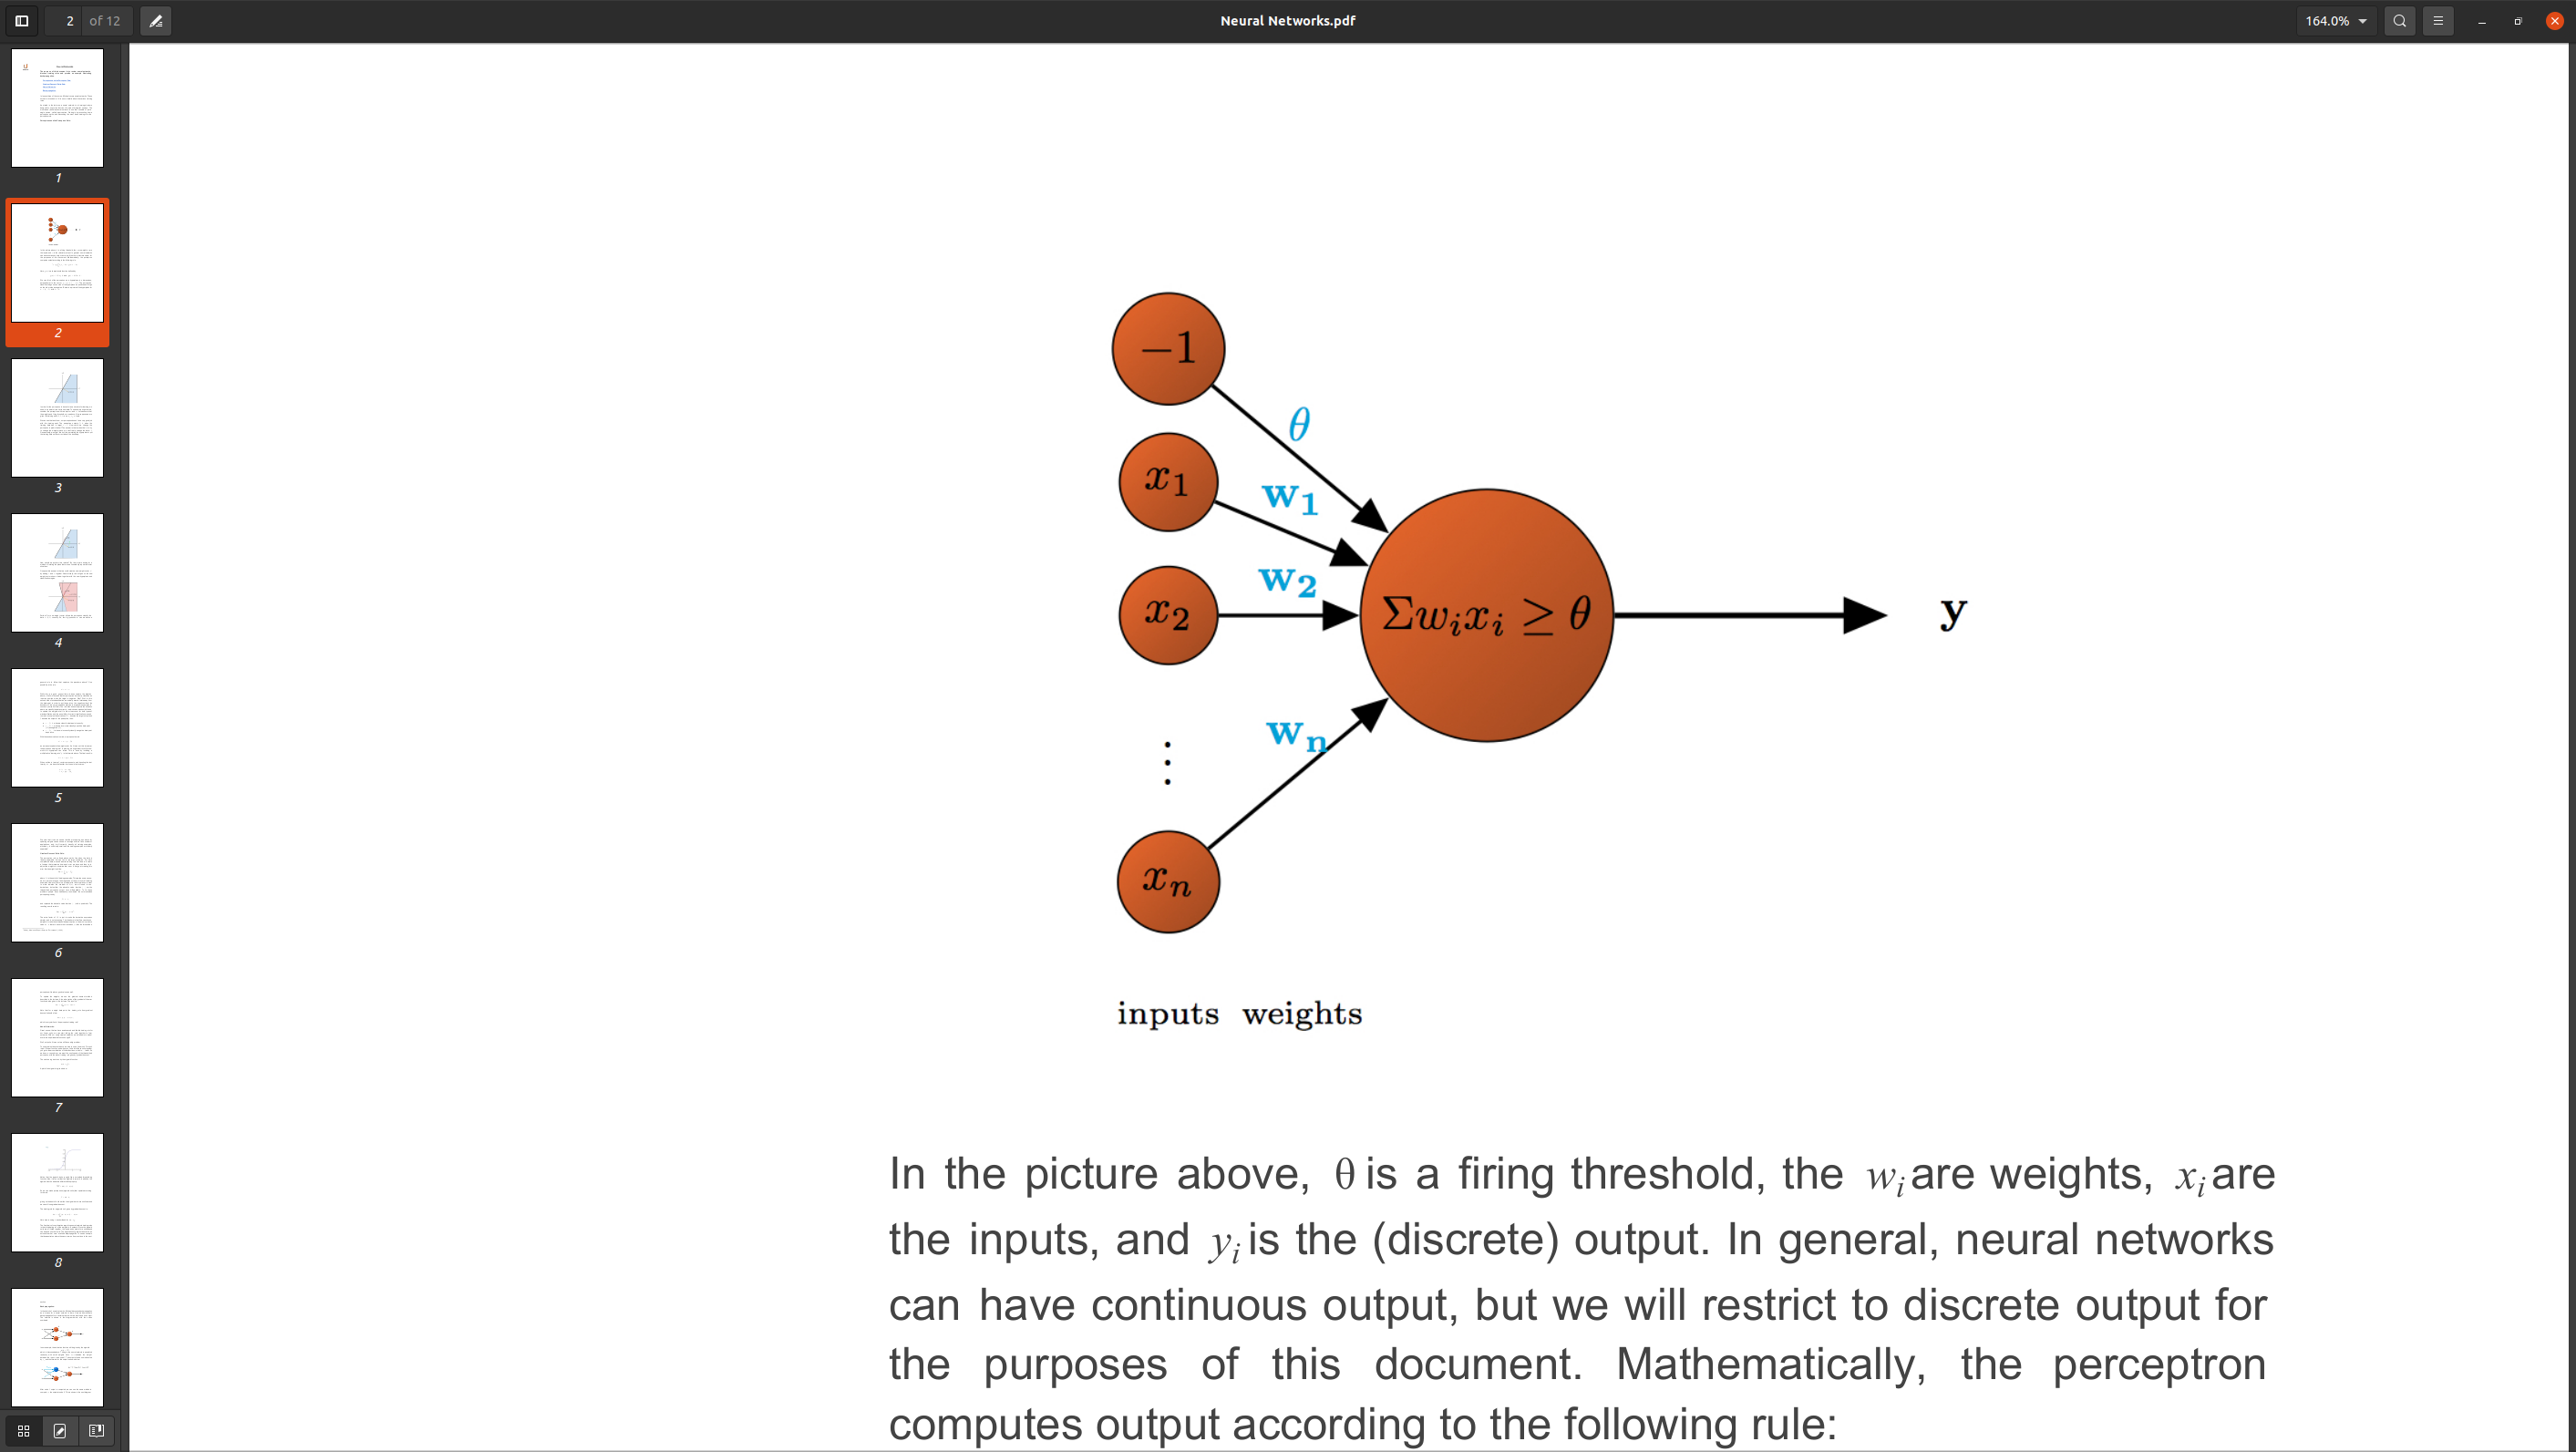
\includegraphics[trim =20cm 15.0cm 10cm 8cm, clip, scale=0.2]{perceptron.png}
	%{\footnotesize\textbf{Notes:} XXX.} % changed <<<<<<<<<<
	%#\label{XXX}
\end{figure}




\section{SL: Instance based learning}
\section{SL: Ensemble B\&B}

Ensemble Learning is in general the process of combining some simple rules into a more complex rule that can generalize well.

It works by dividing the data into smaller subsets, learn over each individual subset to come up with a rule, then combine all these rules in a single more complex rule. If we looked at the whole data, it would be hard to come up with simple rules.




\section{SL: Kernel methods and SVMs}
\section{SL: Comp Learning Theory}
\section{SL: VC dimensions}
\section{SL: Bayesian Learning}
\section{SL: Bayesian inference}


%===============================================================================
%===============================================================================
%===============================================================================
\chapter[Unsupervised learning]{Unsupervised learning (UL)}

\section{Random optimization}
\section{Clustering}

\chapter[Reinforced Learning]{Reinforced Learning (RL)}

\section{Markov Decision Process}

\chapter[Miscellaneous topics]{Miscellaneous topics}

\section{One hot encoding}
\label{sec:one-hot}

\href{https://www.youtube.com/watch?v=v_4KWmkwmsU&ab_channel=deeplizard}{source1} and \href{https://machinelearningmastery.com/how-to-one-hot-encode-sequence-data-in-python/}{source2}

A one hot encoding is a representation of categorical variables as binary vectors. This first requires that the categorical values be mapped to integer values. Then, each integer value is represented as a binary vector that is all zero values except the index of the integer, which is marked with a 1.

Example: assume we have a sequence of labels with the values \textit{red} and \textit{green}. We can assign \textit{red} an integer value of 0 and \textit{green} the integer value of 1. As long as we always assign these numbers to these labels, this is called an integer encoding. Consistency is important so that we can invert the encoding later and get labels back from integer values, such as in the case of making a prediction. Next, we can create a binary vector to represent each integer value. The vector will have a length of 2 for the 2 possible integer values. The \textit{red} label encoded as a 0 will be represented with a binary vector [1, 0] where the zeroth index is marked with a value of 1. In turn, the \textit{green} label encoded as a 1 will be represented with a binary vector [0, 1] where the first index is marked with a value of 1. If we had the sequence: \textit{red, red, green}, we could represent it with the integer encoding: 0, 0, 1. And the one hot encoding of:
[1, 0], [1, 0], and [0, 1].

Why Use a One Hot Encoding?
A one hot encoding allows the representation of categorical data to be more expressive. Many machine learning algorithms cannot work with categorical data directly. The categories must be converted into numbers. This is required for both input and output variables that are categorical. We could use an integer encoding directly, rescaled where needed. This may work for problems where there is a natural ordinal relationship between the categories, and in turn the integer values, such as labels for temperature \textit{cold, warm, and hot}.

There may be problems when there is no ordinal relationship and allowing the representation to lean on any such relationship might be damaging to learning to solve the problem. An example might be the labels dog and cat

In these cases, we would like to give the network more expressive power to learn a probability-like number for each possible label value. This can help in both making the problem easier for the network to model. When a one hot encoding is used for the output variable, it may offer a more nuanced set of predictions than a single label.

We can use libraries such is scikit-learn and keras to encode a categorical feature for ML.

\section{F1 score, precision, and recall}
Refer to \href{https://scikit-learn.org/stable/auto_examples/model_selection/plot_precision_recall.html#precision-recall}{this source.}

Precision (P) is defined as the number of true positives ($T_p$) over the number of true positives plus the number of false positives ($F_p$):
$P = \frac{T_p}{T_p + F_p} $.

Recall    (R) is defined as the number of true positives ($T_p$) over the number of true positives plus the number of false negatives ($F_n$):
$R = \frac{T_p}{T_p + F_n} $.

These quantities are also related to the ($F1$) score, which is defined as the harmonic mean of precision and recall:
$F1 = 2 \frac{R * P}{ P + R } $.

The F1 score can be interpreted as a harmonic mean of the precision and recall, where an F1 score reaches its best value at 1 and worst score at 0.


\section{Overfitting vs underfitting}
This is a phenomenon called overfitting, where a model matches the training data almost perfectly, but does poorly in validation and other new data. On the flip side, if we make our tree very shallow, it doesn't divide up the houses into very distinct groups.

At an extreme, if a tree divides houses into only 2 or 4, each group still has a wide variety of houses. Resulting predictions may be far off for most houses, even in the training data (and it will be bad in validation too for the same reason). When a model fails to capture important distinctions and patterns in the data, so it performs poorly even in training data, that is called underfitting.

Since we care about accuracy on new data, which we estimate from our validation data, we want to find the sweet spot between underfitting and overfitting. Visually, we want the low point of the (red) validation curve in the figure below.


\section{Cost function}
\label{sec:cost}
Let's use the concept of linear regression to discuss the cost function.
Here is the model:

\begin{equation}
	f_{w,b} (x) = wx + b
\end{equation}

$w, b$ are the parameters/coefficients/weights of the model. In ML, parameters of a model are the variables that you can do training in order to improve the model.

\begin{multline}
		\text{data points } \{(x_i, y_i): i=1 ... m \} \\
    \hat{y}^{(i)} = f_{w,b} (x^{(i)}) = wx ^ {(i)} + b \\
\end{multline}

Problem statement: find $w, b$ such that $\hat{y}^{(i)}$ is close to $y^{(i)}$ for all $(x^{(i)}, y^{(i)} )$. $\big(\hat{y}^{(i)}  - y^{(i)} \big) ^2$, the error for one single sample is called the loss function.



To find $w, b$, we form the the cost function:

\begin{multline}
	\text{find $w, b$:} \\
	\text{minimize:  }  J(w ,b) = \frac{1}{2m} \sum_{i=1}^{m} \big(\hat{y}^{(i)}  - y^{(i)} \big) ^2 = \frac{1}{2m} \sum_{i=1}^{m} \big( wx ^ {(i)} + b - y^{(i)} \big) ^2 \\
\end{multline}
m is the to total number of data points. The extra 2 in the denominator is just for convenience. This is the squared error cost function, which is widely used. However, there are other options for the cost functions as well.

\section{Gradient descent (or steepest descent)}
\label{sec:gradient}

An optimization method to minimize any function. Depending on the initial starting point, the method may end up at a different local minimum.

For a cost function $J(p1, p2, ...)$,  we want to find  $p1, p2, ...$ to minimize $J$.

Algorithm:
start with some initial $p1, p2, ...$.
update $p_i$ \textit{simultaneously} until the algorithm converges, meaning you reach a local minimum, where additional iteration does not change the point. It is incorrect to use new values of $p_i$ to update other parameters in the same iteration.
\begin{equation}
  p_i = p_i - \alpha \frac{\partial  }{\partial p_i} J(p_i) \text{for each i}
\end{equation}

The negative is because we want to move in the opposite direction. $\alpha$ is the learning rate (step size). The choice of learning rate affects the efficiency of gradient descent. If it is too small, it converges very slowly. If it is too large (overshoot), may cause divergence and never reaches the minimum. If we are exactly at the minimum, since slope is zero, the value of the learning does not affect the results. Thus, even a fixed learning can reach the minimum.

\textbf{Various types of gradient descent: }

Batch gradient descent: each step of gradient descent uses all the training examples. While this batching provides computation efficiency, it can still have a long processing time for large training datasets as it still needs to store all of the data into memory. Batch gradient descent also usually produces a stable error gradient and convergence, but sometimes that convergence point isn't the most ideal, finding the local minimum versus the global one.

Mini-batch gradient descent updates the parameters using a subset of training samples.


\section{Model validation}

In most (though not all) applications, the relevant measure of model quality is predictive accuracy. In other words, will the model's predictions be close to what actually happens.

There are many metrics for summarizing model quality, but we'll start with one called Mean Absolute Error (also called MAE). With the MAE metric, we take the absolute value of each error. This converts each error to a positive number. We then take the average of those absolute errors. This is our measure of model quality. sklearn has a function, mean\_absolute\_error, to calculate MAE.


Many people make a mistake when measuring predictive accuracy. They make predictions with their training data and compare those predictions to the target values in the training data. This is not valid. The most straightforward way to validate the model is to exclude some data from the model-building process, and then use those to test the model's accuracy on data it hasn't seen before. This data is called validation data.





% Appendix ==========================================================
%\appendices
%\include{appendix_Matrices}


%\renewcommand*{\bibfont}{\footnotesize}  % This command reduces the font size. Comment this for the final draft
%\renewcommand*{\bibfont}{\scriptsize}  % This command reduces the font size. Comment this for the final draft
\addcontentsline{toc}{chapter}{Bibliography}
\bibliographystyle{plain}  				% Here the bibliography  %
\bibliography{reference}        	% is inserted.			     %
\index{bibliography}

\end{document}

